%%=================================================================================
\begin{frame}{Methodology}
  \begin{minipage}{0.49\linewidth}
    For a given systematic source :
    \begin{itemize}
    \item Create distributions of \\ $m_{\gamma\gamma}^{nom}$, $m_{\gamma\gamma}^{up}$, $m_{\gamma \gamma}^{down}$
    \item Fit main parameter of the systematic with DSCB :
      \begin{itemize}
      \item Fit  $m_{\gamma\gamma}$
      \item Free parameter(s) of interest
      \item Fixing $X=\hat{X}^{nom}$
%        \item Fixing secondary parameter to nominal fitted values.
      \end{itemize}
      \item Systematic variation : $\delta_X=\frac{X^{fluct}}{X^{nom}}-1$, $X\in \{\mu , \sigma\}$
      \end{itemize}
    \end{minipage}
    \hfill
    \begin{minipage}{0.49\linewidth}
      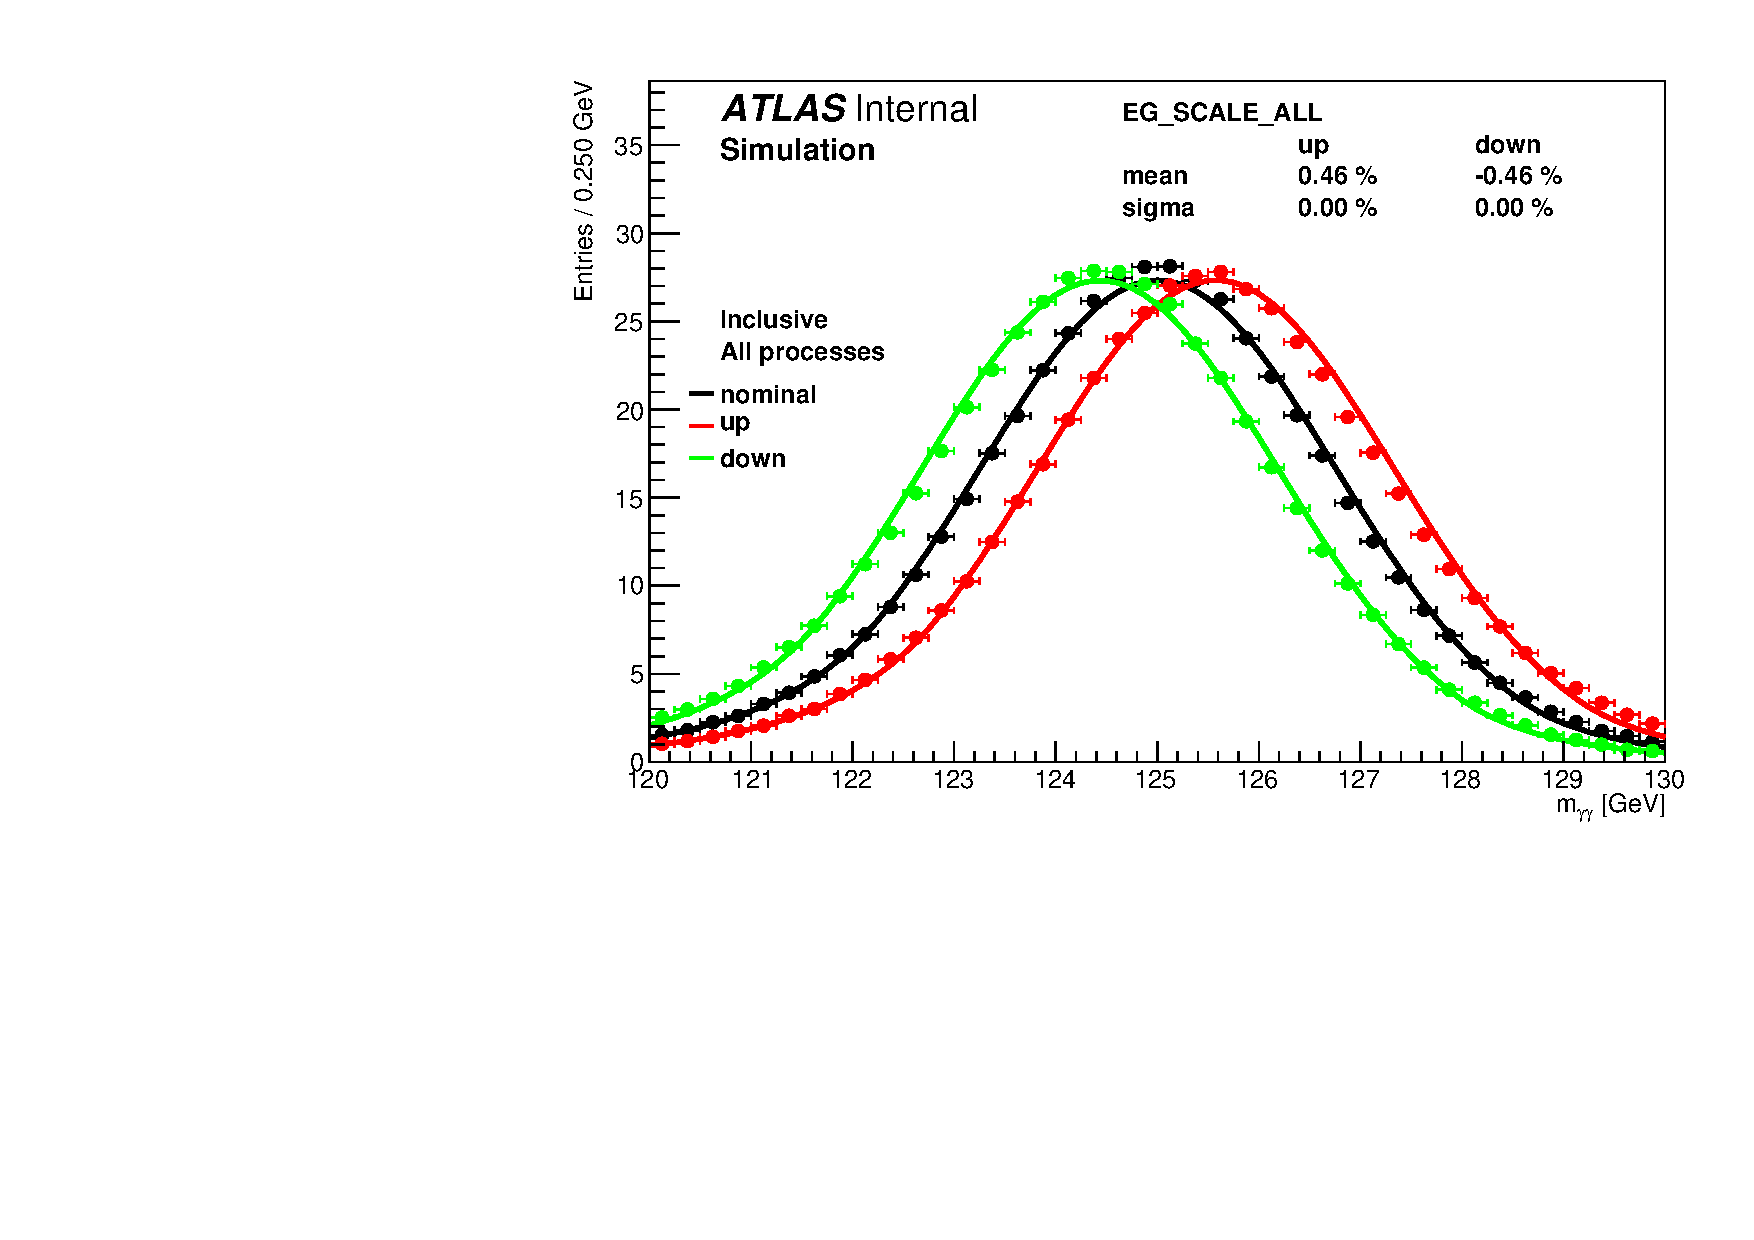
\includegraphics[width=\linewidth]{plots/Backup/h013_EG_SCALE_ALL_0.pdf}
    \end{minipage}
    \vfill
    
    \begin{equation}
      \tiny
      CB(m_{\gamma \gamma}) = 
      \begin{cases}
        e^{-t^{2}/2} & \text{if } -\alpha_{low} \leq t \leq \alpha_{high} \\
        \frac{ e^{-{}^{1}_{2} \alpha_{low}^{2}} } { \left[ \frac{1}{R_{low}} \left(R_{low} - \alpha_{low} - t \right) \right]^{n_{low}} } & \text{if } t < -\alpha_{low} \\
        \frac{ e^{-{}^{1}_{2} \alpha_{high}^{2}} } { \left[ \frac{1}{R_{high}} \left(R_{high} - \alpha_{high} + t \right) \right]^{n_{high}} } & \text{if } t > \alpha_{high} \\
        t=(m_{\gamma\gamma}-\mu)/\sigma, R_{low}=\frac{\alpha_{low}}{n_{low}},  R_{high}=\frac{\alpha_{high}}{n_{high}} \\
      \end{cases}
    \end{equation}
\end{frame}
%%=================================================================================
\begin{frame}{ICHEP Results}
  \begin{minipage}{0.59\linewidth}
    ICHEP results were obtained with only 2 nuisance parameters.\\
    %    \textcolor{red}{Only the fluctuation effects on the POI were considered for the measurement framework.}
    \textcolor{red}{In stat framework, systematic only affects a single dedicated parameter (width or mass).}\\
    \input{plots/h013_ICHEP_PhotonSyst.csv}
    \vfill
  \end{minipage}
  \begin{minipage}{0.4\linewidth}
    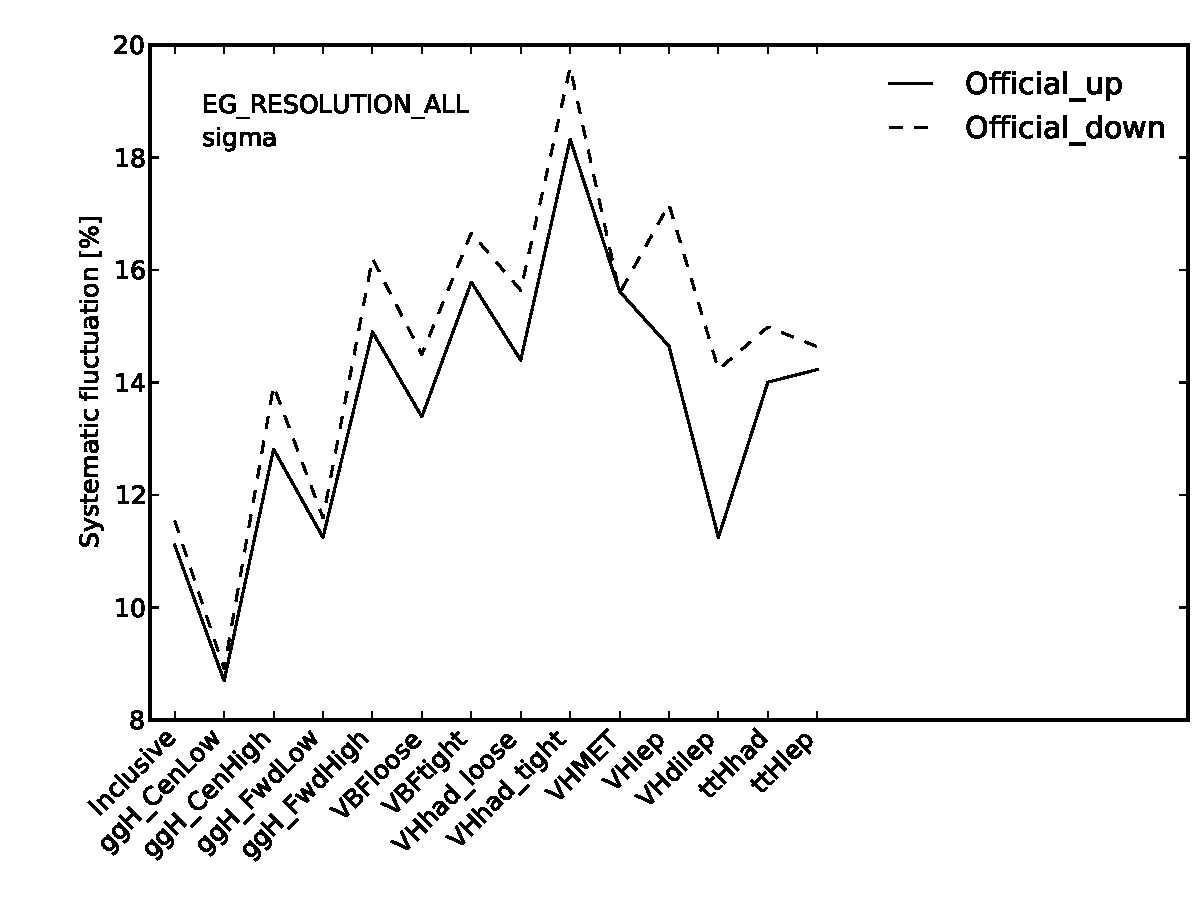
\includegraphics[width=\linewidth]{plots/Backup/h013_ICHEP_PhotonSyst_EG_RESOLUTION_ALL_sigma.pdf}\\
    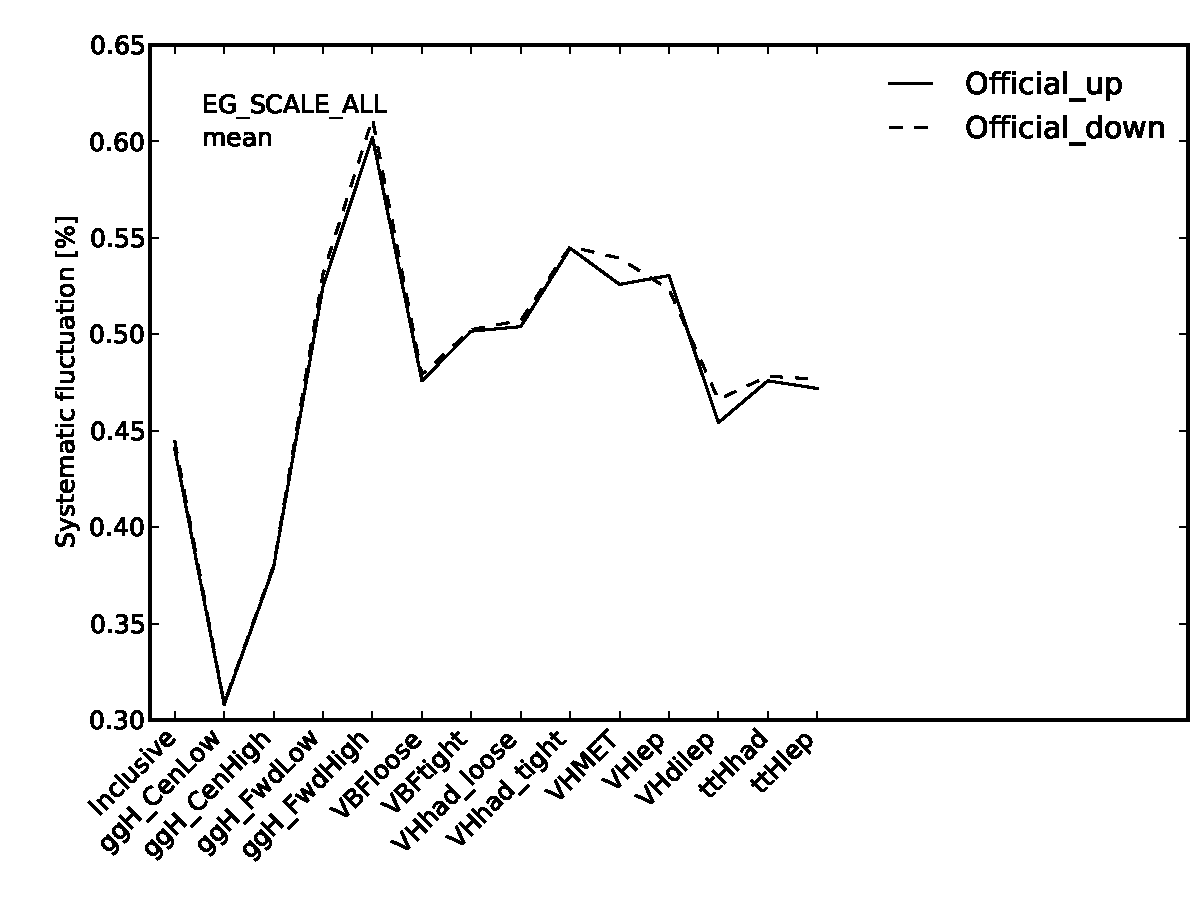
\includegraphics[width=\linewidth]{plots/Backup/h013_ICHEP_PhotonSyst_EG_SCALE_ALL_mean.pdf}\\
  \end{minipage}
\end{frame}

\begin{frame}{Calibration uncertainties contributions}
  \begin{minipage}{0.49\linewidth}
    \includegraphics[width=\linewidth]{/home/goudet/Documents/LAL/ExternalPlot/ATL-COM-PHYS-2016-222_74f.pdf}\\
    \centering
    ATL-COM-PHYS-2016-222
  \end{minipage}
  \begin{minipage}{0.49\linewidth}
    \begin{itemize}
    \item \textcolor{red}{Resolution systematic dominant}
    \item Consequent other experimental contribution
    \item Energy scale has small contribution
    \end{itemize}
  \end{minipage}
\end{frame}

%==============================================================================
\begin{frame}{Scale factors interpretation}
  \begin{minipage}{0.49\linewidth}
    Assume the up fluctuation (red) as data and nominal distribution (black) as MC in the template method.
    One has
    $$m_H^{up}=m_H^{nom}(1+\alpha)$$
    Hence
    $$\delta_{m_H}=\alpha$$
    \end{minipage}
  \begin{minipage}{0.49\linewidth}
    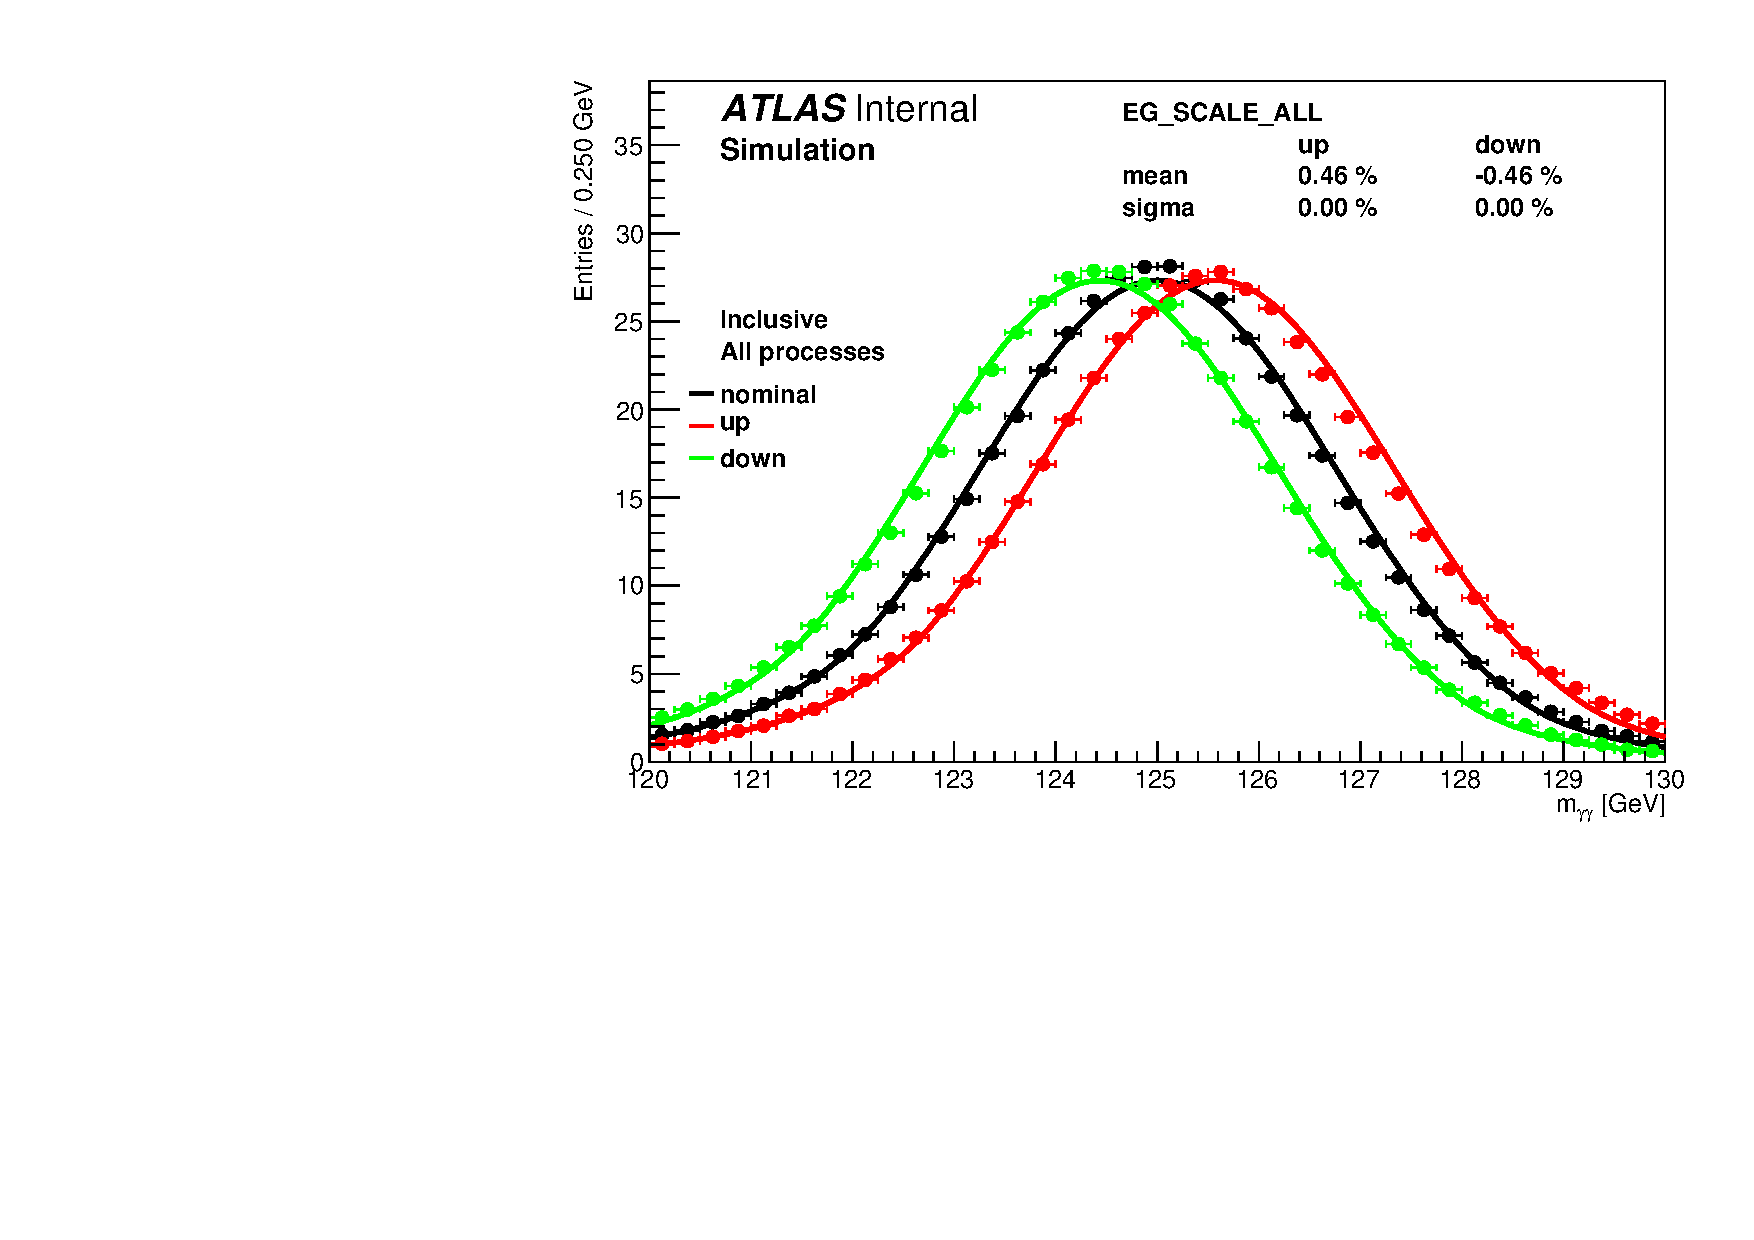
\includegraphics[width=\linewidth]{plots/Backup/h013_EG_SCALE_ALL_0.pdf}
  \end{minipage}
  Furthermore :
  $$\sigma_H^{up}=\sigma_H^{nom} \oplus cE$$
  Hence
  $$\delta_{\sigma_H} = \sqrt{1+\frac{c^2E^2}{\sigma_H^2}}-1$$
  One has to be carefull with resolution uncertainty as the template method is weak to measure small differences.
\end{frame}
